% --------------------------------------------------------------
% This is all preamble stuff that you don't have to worry about.
% Head down to where it says "Start here"
% --------------------------------------------------------------

\documentclass[12pt]{article}

\usepackage[margin=1in]{geometry}
\usepackage{amsmath,amsthm,amssymb}
\usepackage{tikz}
\usepackage{mathtools}
\DeclarePairedDelimiter{\ceil}{\lceil}{\rceil}

\usetikzlibrary{arrows}

\newcommand{\N}{\mathbb{N}}
\newcommand{\Z}{\mathbb{Z}}

\newenvironment{theorem}[2][Theorem]{\begin{trivlist}
\item[\hskip \labelsep {\bfseries #1}\hskip \labelsep {\bfseries #2.}]}{\end{trivlist}}
\newenvironment{lemma}[2][Lemma]{\begin{trivlist}
\item[\hskip \labelsep {\bfseries #1}\hskip \labelsep {\bfseries #2.}]}{\end{trivlist}}
\newenvironment{exercise}[2][Exercise]{\begin{trivlist}
\item[\hskip \labelsep {\bfseries #1}\hskip \labelsep {\bfseries #2.}]}{\end{trivlist}}
\newenvironment{question}[2][Question]{\begin{trivlist}
\item[\hskip \labelsep {\bfseries #1}\hskip \labelsep {\bfseries #2.}]}{\end{trivlist}}
\newenvironment{proposition}[2][Proposition]{\begin{trivlist}
\item[\hskip \labelsep {\bfseries #1}\hskip \labelsep {\bfseries #2.}]}{\end{trivlist}}
\newenvironment{corollary}[2][Corollary]{\begin{trivlist}
\item[\hskip \labelsep {\bfseries #1}\hskip \labelsep {\bfseries #2.}]}{\end{trivlist}}

\begin{document}

% --------------------------------------------------------------
%                         Start here
% --------------------------------------------------------------

%\renewcommand{\qedsymbol}{\filledbox}

\title{Homework 5}%replace X with the appropriate number
\author{Dustin Lambright - dalambri \\ Aseem Raina - araina \\ Bihan Zhang - bzhang28 \\ Anshul Fadnavis - asfadnav\\
%replace with your name
CSC 565 - Graph Theory} %if necessary, replace with your course title

\maketitle


\begin{question}{1}
Problem 4.1.8, text. For each $k$, which graphs are $k$-connected? Which are $k$-edge connected?
\end{question}

\noindent
The Hexagon \\
$\kappa$: 4 \\
$\kappa$':4 \\
$\delta$: 4 \\
4-connected? Yes \\
4-edge-connected? Yes  \\
The Other one \\
$\kappa$: 2 \\
$\kappa$':4 \\
$\delta$: 4 \\
4-connected? Yes \\
4-edge-connected? Yes

\begin{question}{2}
For $k \leq n - 1$, prove that every simple $n$-vertex graph $G$ with $\delta(G) \geq (n+k-2)/2$ is $k$-connected.
\end{question}

PROOF BY INDUCTION: \\
Start with $n$ = 1. Since $n = 1, k = 0$. A single node is $K_1$, and $K_1$ is $0$-connected by virtue of the $K$-graph rule. \\

Increment $n$:
As $n$ increases, so will $\delta$.  $\delta$ also increases. For $n = 2, k =0, \delta = \frac{2}{2}$.  The Harary graph $H_{2}{1}$, the graph with the fewest possible edges to achieve $\delta = k$ is 1-connected, therefore 0-connected.  $\delta$ will increase by 1 for every other increment of $k$. As $n$ increases, we build a Harary graph $H_{(n)(k)}$, which will be k-connected.  This will be the case for every $H_{(n)(k)}$.

\begin{question}{3}

($!$) Prove that the symmetric difference of two different edge cuts is an edge cut. (Hint: Draw a picture illustrating the two edge cuts and use it to guide the proof.)

	4.1.28 Text \\
	The symmetric difference of $[X,\bar{X}]$ and $[Y,\bar{Y}]$ is the edge cut \\
	$[Z,\overline{Z}] = [(X \cap Y) \cup (\overline{X} \cap \overline{Y}), (X \cap \overline{Y}) \cup (\overline{X} \cap Y)]$\\
	
	An edge e is only in $[Z, \overline{Z}]$ if it is in exactly one of $[X,\overline{X}]$ or $[Y, \overline{Y}]$
	
	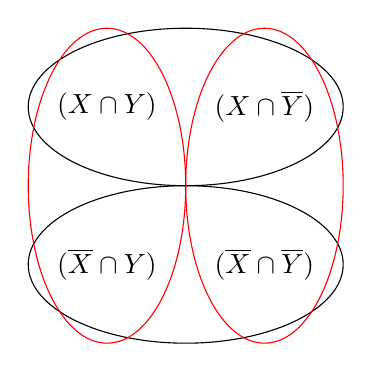
\begin{tikzpicture}
	\draw (0,0) ellipse (2cm and 1cm);
	\draw (0,2) ellipse (2cm and 1cm);
	\draw[red] (-1,1) ellipse (1cm and 2cm);
	\draw[red] (1,1) ellipse (1cm and 2cm);
	\node at (-1,2){$(X \cap Y)$};
	\node at (1,0){$(\overline{X} \cap \overline{Y})$};
	\node at (1,2){$(X \cap \overline{Y})$};
	\node at (-1,0){$(\overline{X} \cap Y)$};
	\end{tikzpicture}
	
\end{question}

\begin{question}{4}
($-$) Let $G$ be the simple graph with vertex set \{1...11\} defined by $i \leftrightarrow j$ if and only if $i, j$ have a common factor bigger than 1.  Determine the blocks of $G$.
\begin{align*}
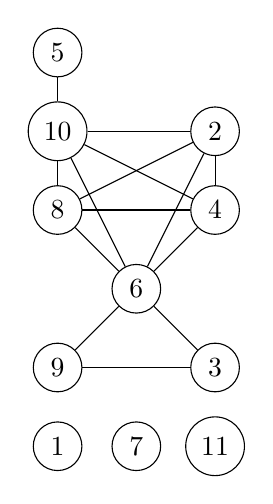
\begin{tikzpicture}
\node[shape=circle,draw=black] (A) at (0,5) {5};
\node[shape=circle,draw=black] (B) at (0,4) {10};
\node[shape=circle,draw=black] (C) at (2,4) {2};
\node[shape=circle,draw=black] (D) at (0,3) {8};
\node[shape=circle,draw=black] (E) at (2,3) {4};
\node[shape=circle,draw=black] (F) at (1,2) {6};
\node[shape=circle,draw=black] (G) at (0,1) {9};
\node[shape=circle,draw=black] (H) at (2,1) {3};
\node[shape=circle,draw=black] (I) at (0,0) {1};
\node[shape=circle,draw=black] (I) at (1,0) {7};
\node[shape=circle,draw=black] (I) at (2,0) {11};
\path [] (A) edge node[left] {} (B);
\path [] (B) edge node[left] {} (C);
\path [] (B) edge node[left] {} (D);
\path [] (B) edge node[left] {} (E);
\path [] (B) edge node[left] {} (F);
\path [] (C) edge node[left] {} (D);
\path [] (C) edge node[left] {} (E);
\path [] (C) edge node[left] {} (F);
\path [] (D) edge node[left] {} (E);
\path [] (D) edge node[left] {} (F);
\path [] (E) edge node[left] {} (F);
\path [] (F) edge node[left] {} (G);
\path [] (F) edge node[left] {} (H);
\path [] (G) edge node[left] {} (H);
\end{tikzpicture}
\end{align*}

The blocks are: $V(5, 10) $, $V(6,9,3)$, $V(1)$, $V(7)$, $V(11)$, $V(10,2,4,6,8)$
\end{question}

\begin{question}{5}
	Give a formula for the number of spanning trees of G in terms of the number of spanning trees of its blocks.	\\
	$\tau(G) = \prod{\tau(\text{Blocks})}$\\
	This is because:\\
	- The graph can be decomposed into its blocks\\
	- Any combination of spanning trees of all blocks will still leave the resultant graph (now a spanning tree) connected, as long as the original graph is connected.
\end{question}

\begin{question}{6}
($-$) Determine $\kappa(u,v)$ and $\kappa`(u,v)$ in the graph drawn below. (Hint: Use the dual problems to give short proofs of optimality)

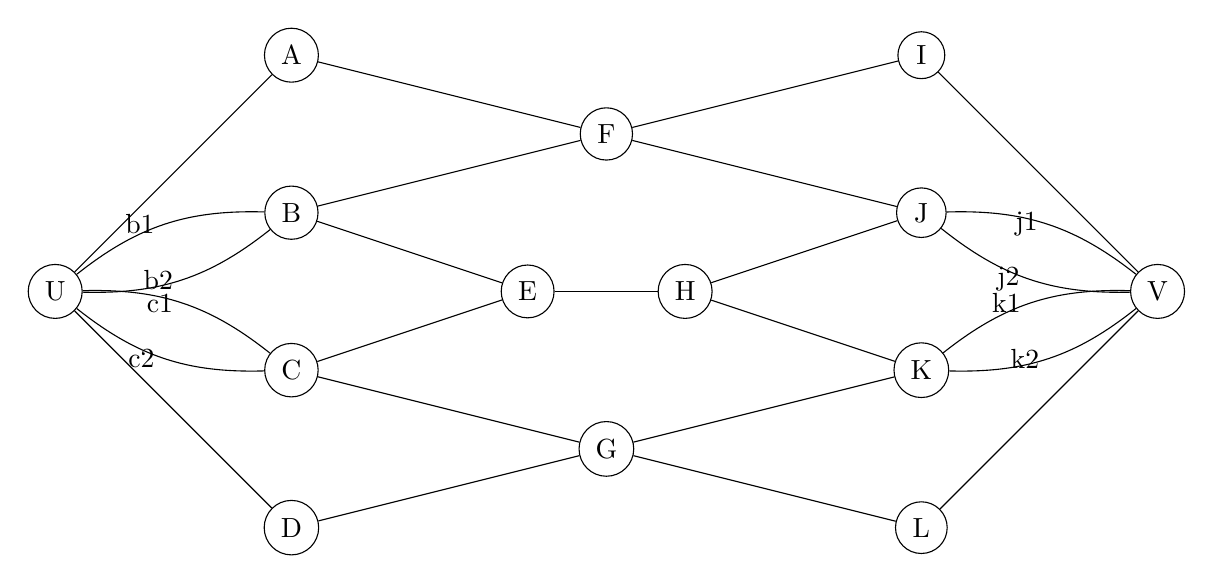
\begin{tikzpicture}
\tikzset{edge/.style = {->,> = latex'}}

\node[shape=circle,draw=black] (U) at (0,3) {U};
\node[shape=circle,draw=black] (A) at (3,6) {A};
\node[shape=circle,draw=black] (B) at (3,4) {B};
\node[shape=circle,draw=black] (C) at (3,2) {C};
\node[shape=circle,draw=black] (D) at (3,0) {D};
\node[shape=circle,draw=black] (E) at (6,3) {E};
\node[shape=circle,draw=black] (F) at (7,5) {F};
\node[shape=circle,draw=black] (G) at (7,1) {G};
\node[shape=circle,draw=black] (H) at (8,3) {H};
\node[shape=circle,draw=black] (I) at (11,6) {I};
\node[shape=circle,draw=black] (J) at (11,4) {J};
\node[shape=circle,draw=black] (K) at (11,2) {K};
\node[shape=circle,draw=black] (L) at (11,0) {L};
\node[shape=circle,draw=black] (V) at (14,3) {V};

\path [] (U) edge node[left] {} (A);
\path [] (U) edge [bend left=20] node[left] {b1} (B);
\path [] (U) edge [bend right=20] node[left] {b2} (B);
\path [] (U) edge [bend left=20] node[left] {c1} (C);
\path [] (U) edge [bend right=20] node[left] {c2} (C);
\path [] (U) edge node[left] {} (D);
\path [] (A) edge node[left] {} (F);
\path [] (B) edge node[left] {} (F);
\path [] (B) edge node[left] {} (E);
\path [] (C) edge node[left] {} (E);
\path [] (C) edge node[left] {} (G);
\path [] (D) edge node[left] {} (G);
\path [] (E) edge node[left] {} (H);
\path [] (F) edge node[left] {} (I);
\path [] (F) edge node[left] {} (J);
\path [] (G) edge node[left] {} (K);
\path [] (G) edge node[left] {} (L);
\path [] (H) edge node[left] {} (J);
\path [] (H) edge node[left] {} (K);
\path [] (I) edge node[left] {} (V);
\path [] (J) edge [bend left=20] node[left] {j1} (V);
\path [] (J) edge [bend right=20] node[left] {j2} (V);
\path [] (K) edge [bend left=20] node[left] {k1} (V);
\path [] (K) edge [bend right=20] node[left] {k2} (V);
\path [] (L) edge node[left] {} (V);
\end{tikzpicture}
\\
For the given graph (with nodes and some edges annotated for convenience):\\
\\
$\kappa(u, v) = 3$\\
For proof of optimality, we could use the duality:\\
$\kappa(u, v) = $ number of vertex-disjoint paths between $u$ and $v$, which are the following:\\
$u-A-F-I-v$\\
$u-B-E-H-J-v$\\
$u-C-G-K-v$\\
In other words, all $u-v$ paths must contain at least one of F, E or G.\\
\\
$\kappa'(u, v) = 5$\\
For proof of optimality, we could use the duality:\\
$\kappa'(u, v) = $ number of edge-disjoint paths between $u$ and $v$, which are the following:\\
$uA-AF-FI-Iv$\\
$b1-BF-FJ-j1$\\
$b2-BE-EH-HJ-j2$\\
$c1-CG-GK-k1$\\
$uD-DG-GL-Lv$\\
In other words, all $u-v$ paths must contain at least one of $AF, BF, EH, CG$ or $DG$.\\

\end{question}

\begin{question}{7}
Prove that a simple graph $G$ is 2-connected if and only if for every triple $(x, y, z)$ of distinct vertices, $G$ has an $x, z$ path through $y$.
\end{question}

\begin{question}{8}
Prove that if $\kappa(G) = k$ and diam($G) = d$, then $n(G) \geq k(d$ - $ 1) + 2$ and $\alpha(G) \geq \ceil[big]{(1 + d)/2}$.
\\
Given graph $G$ with diameter $d$, there exists two vertices $a$ and $b$ with a shortest path between them consisting of at most ($d$ - $1$) edges.  If $\kappa(G) = k$, then there exist $k$ vertex-disjoint paths between $a$ and $b$ of length $\geq (d$ - $1)$, since there cannot be a path shorter than $(d$ - $1)$ between $a$ and $b$, because that path would be the diameter.  These $k$ paths share points $a$ and $b$, adding 2 to the minimum number of vertices.  The end result is $n(G) \geq k(d$ -$1) +2$.  \\

\noindent
Given a graph $G$ with diameter $d$, we can infer that there is a path with $d+1$ vertices that created the diameter.  This path will be isomorphic to $P_{d+1}$.  The maximum independent set will have at least $\ceil[big]{(1 + d)/2}$ vertices on the diameter alone.  Any additional vertices can only increase the size of $\alpha$.



\end{question}

\begin{question}{9}
In a network $N$, with source $s$ and sink $t$, prove that if there exists no directed ($s, t$)-path then the value of a maximum flow and the capacity of a minimum cut are both zero. (goal: short, elegant, correct proof) \\

If we run the Ford-Fulkerson Algorithm on a graph with no directed (s,t)-path from source to sync, the algorithm will not find a f-augmenting path (since it can only reach t by using backwards edges whose value is the 0 flow), it would return a [S,$\bar{S}$] edge cut with 0 capacity (since the algorithm is initialized with every flow(0)). Thus the maximum flow is also 0.
\end{question}

\begin{question}{10}
($-$) A kitchen sink draws water from two tanks according to the network of pipes with capacities per unit time shown below.  Find the maximum flow.  Prove that your answer is optimal by using the dual problem, and explain why this proves optimality.\\

%In every network, the maximum feasible flow is equivalent to the minimum capacity of a source/sink cut by Corollary 4.3.8. The maximum feasible flow in this case is 34, because the edge cut \{Tank1, Tank2, B\} and \{A, C, D, E, F\} produces the minimum capacity 34. Every other cut has a greater capacity. \\
	
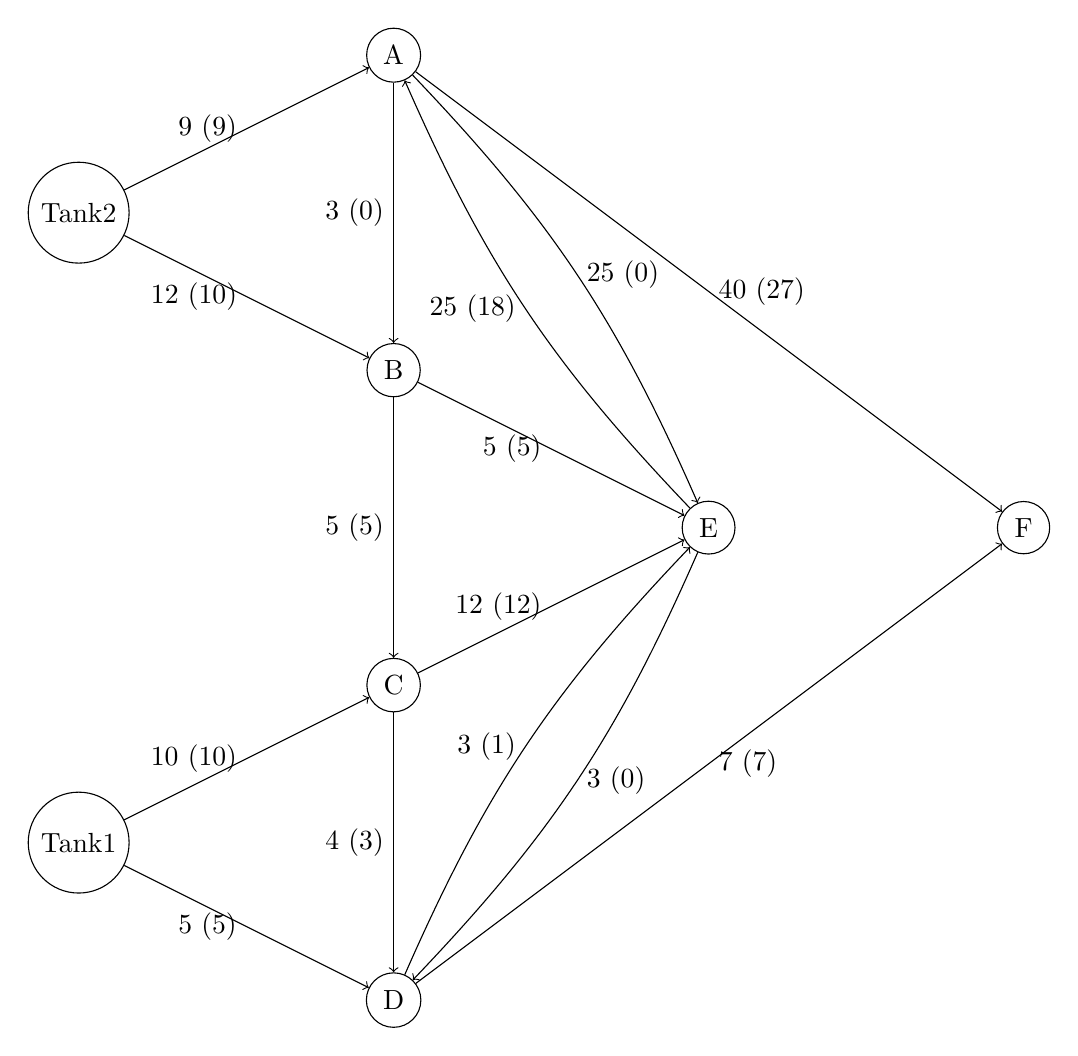
\begin{tikzpicture}
\tikzset{edge/.style = {->,> = latex'}}

\node[shape=circle,draw=black] (A) at (0,10) {Tank2};
\node[shape=circle,draw=black] (B) at (0,2) {Tank1};
\node[shape=circle,draw=black] (C) at (4,12) {A};
\node[shape=circle,draw=black] (D) at (4,8) {B};
\node[shape=circle,draw=black] (E) at (4,4) {C};
\node[shape=circle,draw=black] (F) at (4,0) {D};
\node[shape=circle,draw=black] (G) at (8,6) {E};
\node[shape=circle,draw=black] (H) at (12,6) {F};

\path [->] 

(A)	edge[] node[left] {9 (9)} (C)
(A) edge[] node[left] {12 (10)} (D)
(B) edge[] node[left] {10 (10)} (E)
(B) edge[] node[left] {5 (5)} (F)
(C) edge[] node[left] {3 (0)} (D)
(D) edge[] node[left] {5 (5)} (E)
(E) edge[] node[left] {4 (3)} (F)
(C) edge[bend left=10] node[right] {25 (0)} (G)
(G) edge[bend left=10] node[left] {25 (18)} (C)
(D) edge[] node[left] {5 (5)} (G)
(E) edge[] node[left] {12 (12)} (G)
(F) edge[bend left=10] node[left] {3 (1)} (G)
(G) edge[bend left=10] node[right] {3 (0)} (F)
(C) edge[] node[right] {40 (27)} (H)
(F) edge[] node[right] {7 (7)} (H)
;

\end{tikzpicture}

\end{question}




% --------------------------------------------------------------
%     You don't have to mess with anything below this line.
% --------------------------------------------------------------

\end{document}
